\providecommand{\main}{..}

\documentclass[/home/francois/latex/report/main.tex]{subfiles}

\begin{document}

\chapter{Method}
\label{chapter:method}

This chapter presents the inertial parameters estimation approach starting from the global strategy and continuing with a detailed description of the essential parts of the methods including:

\begin{itemize}
  \item Signal Pre-processing
  \item Tool Inertial Parameters Estimation
  \item Objective Function Computation
\end{itemize}

\section{Signal Pre-processing}

In the chaper \ref{chapter:background}, two models of the \{item\} and \{tool\} systems have been developed. The purpose is to compute the matrices of the equation and then use one or another optimization process. The matrices $A$ and $B$ (respectively $A'$ and $B'$) are computed out of the \ac{FT} sensor measurement and the position and orientation of the \ac{TCP}. One point must be made: signals cannot be merely input in the optimization procedures. Both \ac{FT} measurements and simple method for derivation leads to noisy signals. Consequently, measured signals have to be pre-processed.

\subsection{\textsc{Euler}'s angles continuity filter}

The input orientation of the \ac{TCP} is expressed as \ac{RPY} \textsc{Euler}'s angles. Thus, they are computed in a range of $[]-\pi, \pi]$. Approaching to the interval limit (cf. \ref{section:results:pre-processing}), the signal jumps from positive to negative $\pi$. In addition, the representation by \textsc{Euler}'s angles has no unicity because it depends on the order of axes (anisotropy). When deriving the angular speed and angular acceleration, the outcome is consequently unsatisfying. To tackle that unicity issue, the great properties of quaternion conversion are applied to the set of angles. Subsenquently, the \ac{RPY} angles are filtered with a continuity algorithm (cf. Algorithm \ref{alg:method:continuity}).

The quaternion filter consists in three steps:

\begin{itemize}
  \item convert the \textsc{Euler}'s angles to quaternion,
  \item compute the rotation matrix out of the quaternion vector,
  \item convert the rotation matrix to a \ac{RPY} set of angle.
\end{itemize}

\begin{algorithm}
\caption{Make a \textsc{Euler}'s angles signal continuous\label{alg:method:continuity}}
\begin{algorithmic}
\FOR{\texttt{orientation} in \texttt{signal}}
 \FOR{\texttt{angle} in \texttt{orientation}}
  \STATE \texttt{previous}  $\leftarrow$ \texttt{current}
  \STATE \texttt{current}  $\leftarrow$ \texttt{angle}
  \IF{$\text{\texttt{current}} \times \text{\texttt{previous}} < 0$}
   \IF{$\text{\texttt{current}} - \text{\texttt{previous}} > 0$}
    \STATE $\text{\texttt{angle}} \leftarrow \text{\texttt{current}} - 2 \pi$
   \ELSE
    \STATE $\text{\texttt{angle}} \leftarrow \text{\texttt{current}} + 2 \pi$
   \ENDIF
  \ENDIF
 \ENDFOR
\ENDFOR
\end{algorithmic}
\end{algorithm}

\subsection{\textsc{Savitzky–Golay} filter}

Therefore, it is needed to derived the linear and angular velocity and the linear and angular speed from the \ac{TCP} pose. First tests conducted with simple derivation method using $f'(t) \approx  [f(t+\delta) - f(t)] / \delta$ does not provide good results (cf. comparison in \ref{section:results:pre-processing}). The noise induced in the \ac{TCP} pose measurement generates spikes in the derivated signal. One approach is to use \textsc{Savitzky–Golay} filter to guatantee smooth derivated signals.

The method was created in 1964 by A. \textsc{Savitzky} M. J. E. \textsc{Golay} \cite{Savitzky1964} in their seminal article. The smoothing of a signal or its derivative is achieved with a convolution process. Sub-sets of adjacent data points are fitted to a low-degree polynomial by the method of linear \ac{LS} (cf. \ref{fig:method:savit}). Convoluation coefficients are then use to give estimates of the smoothed signal, (or derivatives of the smoothed signal) at the central point of each sub-set.

\begin{figure}
  \centering
  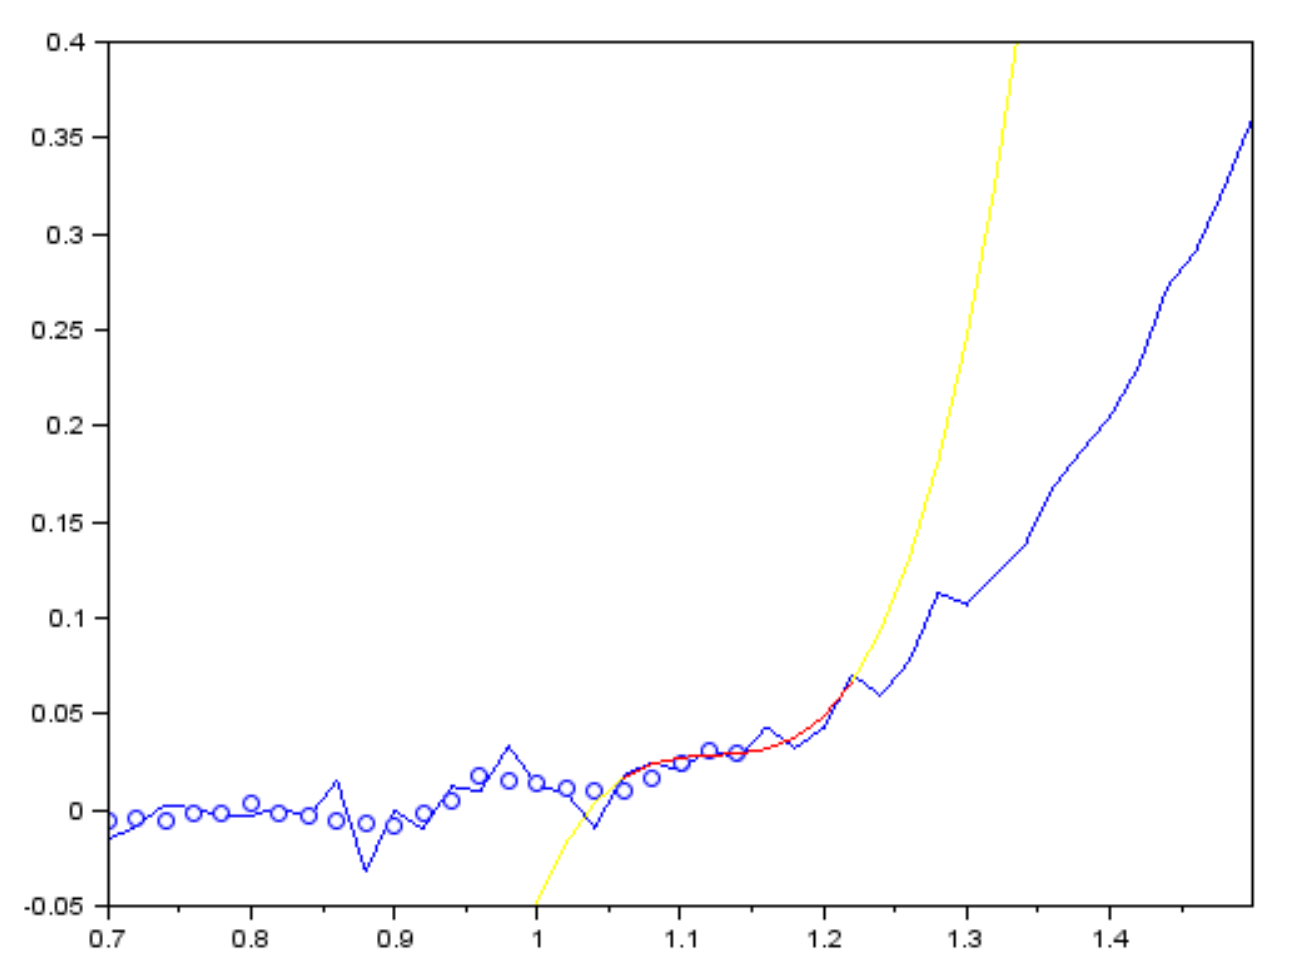
\includegraphics[scale=0.25]{\main/figures/savitzky-golay-filter.png}
  \caption{Smoothing of noisy data by the \textsc{Savitzky–Golay} method ($3^{rd}$ degree polynomial, 9 points wide sliding window). Blue curve: raw data; blue circle: point after smoothing; yellow curve: polynomial used to determine the current point; red curve: polynomial restricted to the sliding window around the current point. Image from \cite{Cdang2013}.}
  \label{fig:method:savit}
\end{figure}

\subsection{Low-pass filter}

As mentioned above, the \ac{FT} signal is slightly noisy. As the frequency of the noise is relatively high, it is considered to use a low-pass filter. The choice fell on the \textsc{Butterworth} filter (cf. \cite{filter1923}), a signal processing filter which is having a flat frequency response in the passband can be termed as Butterworth filter and is also called as a maximally flat magnitude filter (cf. \ref{fig:method:butter}).

Besides, this low-pass filter is applied twice, once forward and once backwards. The combined filter has zero phase and a filter order twice that of the original \cite{SciPy2019}.

\begin{figure}
  \centering
  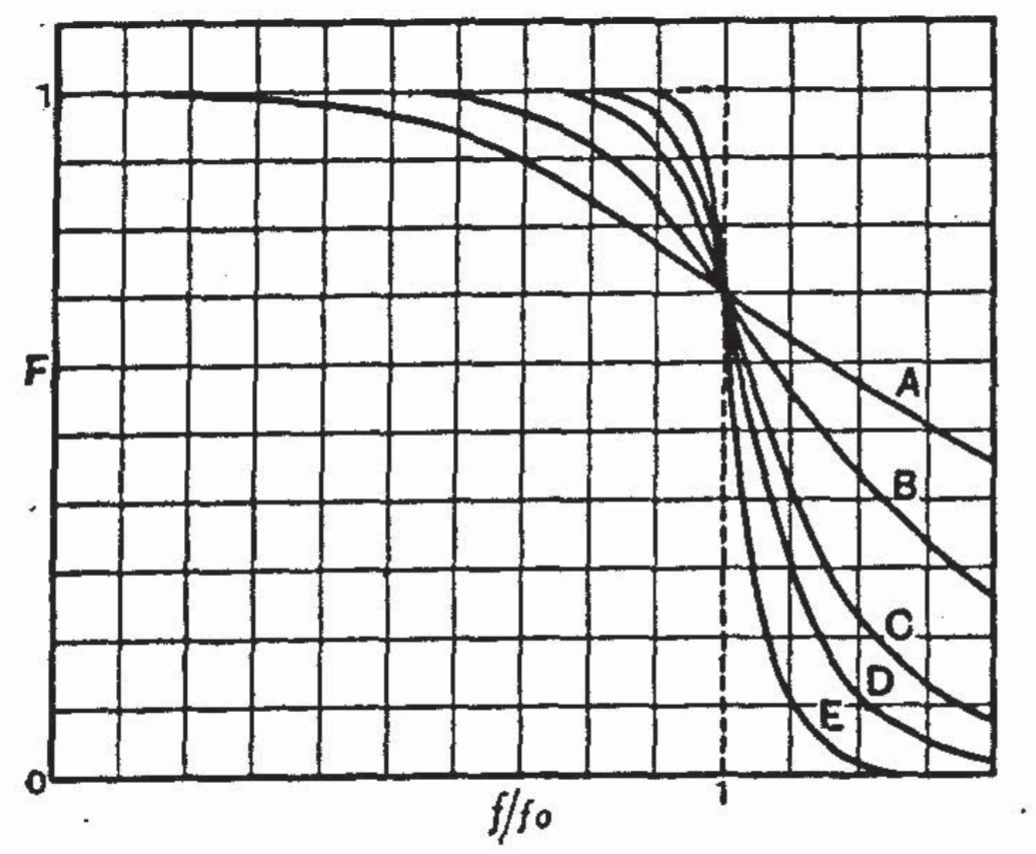
\includegraphics[scale=0.25]{\main/figures/butter.png}
  \caption{Frequency response plot from different order \textsc{Butterworth} filter. Image from  \cite{filter1923}.}
  \label{fig:method:butter}
\end{figure}

\section{Estimating the robotic manipulator tool parameters}

\textit{TODO}



{\it
Estimation of the general dynamic parameters:

\begin{itemize}
  \item tool parameters: mass $m_t$, center of mass $c_t$, moment of inertia $I_t$
  \item suction cup parameters: spring coefficient $K$, damping ratio $\Lambda$.
\end{itemize}
}

\section{Inertial parameters estimation strategy}

\textit{TODO}

{\it
Estimation of the inertial parameters of the item:

\begin{itemize}
  \item off-line method
  \item on-line method
\end{itemize}
}

\begin{figure}[H]
\centering
   % % \documentclass[tikz]{standalone}

% \usetikzlibrary{shapes,arrows,shadows}
% \usepackage{amsmath,bm,times}
% \newcommand{\mx}[1]{\mathbf{\bm{#1}}} % Matrix command
% \newcommand{\vc}[1]{\mathbf{\bm{#1}}} % Vector command
%%%%%%%%%%%%%%%%%%%%%%%%%%%%%%%%%%%%
%%% BEGIN DOCUMENT
% \begin{document}

\pgfdeclarelayer{background}
\pgfdeclarelayer{foreground}
\pgfsetlayers{background,main,foreground}

% Define block styles used later

\tikzstyle{sensor}=[draw, fill=blue!20, text width=5em,
    text centered, minimum height=2.5em,drop shadow]
\tikzstyle{ann} = [above, text width=5em, text centered]
\tikzstyle{wa} = [sensor, text width=10em, fill=red!20,
    minimum height=6em, rounded corners, drop shadow]
\tikzstyle{sc} = [sensor, text width=13em, fill=red!20,
    minimum height=10em, rounded corners, drop shadow]

% Define distances for bordering
\def\blockdist{2.3}
\def\edgedist{2.5}

\begin{tikzpicture}
    \node (wa) [wa]  {System Combination};
    \path (wa.west)+(-3.2,1.5) node (asr1) [sensor] {$ASR_1$};
    \path (wa.west)+(-3.2,0.5) node (asr2)[sensor] {$ASR_2$};
    \path (wa.west)+(-3.2,-1.0) node (dots)[ann] {$\vdots$};
    \path (wa.west)+(-3.2,-2.0) node (asr3)[sensor] {$ASR_N$};

    \path (wa.east)+(\blockdist,0) node (vote) [sensor] {$\theta_0,\theta_1,...,\theta_M$\\Estimated Parameters};

    \path [draw, ->] (asr1.east) -- node [above] {}
        (wa.160) ;
    \path [draw, ->] (asr2.east) -- node [above] {}
        (wa.180);
    \path [draw, ->] (asr3.east) -- node [above] {}
        (wa.200);
    \path [draw, ->] (wa.east) -- node [above] {}
        (vote.west);


    \path (wa.south) +(0,-\blockdist) node (asrs) {System Combination - Training};

    \begin{pgfonlayer}{background}
        \path (asr1.west |- asr1.north)+(-0.5,0.3) node (a) {};
        \path (wa.south -| wa.east)+(+0.5,-0.3) node (b) {};
        \path (vote.east |- asrs.east)+(+0.5,-0.5) node (c) {};

        \path[fill=yellow!20,rounded corners, draw=black!50, dashed]
            (a) rectangle (c);
        \path (asr1.north west)+(-0.2,0.2) node (a) {};

    \end{pgfonlayer}

    % Validation Layer is the same except that there are a set of nodes and links which are added


    \path (wa.south)+(-2.0,-7.5) node (syscomb) [sc] {\textbf{System Combination \\Algorithm}\\Estimated Parameters\\from training};
    \path (syscomb.west)+(-2.2,1.5) node (asrt1) [sensor] {$ASR_1$};
    \path (syscomb.west)+(-2.2,0.5) node (asrt2)[sensor] {$ASR_2$};
    \path (syscomb.west)+(-2.2,-1.0) node (dots)[ann] {$\vdots$};
    \path (syscomb.west)+(-2.2,-2.0) node (asrt3)[sensor] {$ASR_N$};

    \path [draw, ->] (asrt1.east) -- node [above] {}
        (syscomb.160) ;
    \path [draw, ->] (asrt2.east) -- node [above] {}
        (syscomb.180);
    \path [draw, ->] (asrt3.east) -- node [above] {}
        (syscomb.200);


    \path (wa.south) +(0,-\blockdist) node (sct) {System Combination - Training};


    \path (syscomb.east)+(1.0,0.0) node (bwtn) {};

    % Note how the single nodes are repeated using for loop
    \foreach \x in {0,1,...,4}
    {
        \draw (bwtn.east)+(\x,0) node (asr\x-2)[]{};
        \fill (bwtn.east)+(\x,0) circle (0.1cm);
    }

    \path [draw, ->] (syscomb.east) -- node [above] {}
        (bwtn.east);
	\path [draw, ->] (asr0-2) -- node [above] {@}
        (asr1-2);
    \path [draw, -] (asr1-2) -- node [above] {b}
        (asr2-2);
    \path [draw, -] (asr2-2) -- node [above] {z}
        (asr3-2);
    \path [draw, -] (asr3-2) -- node [above] {}
        (asr4-2);

    \path [draw, ->] (asr0-2) edge[bend  right]  node [below] {@}
        (asr1-2);
    \path [draw, ->] (asr1-2) edge[bend  right]  node [below] {b}
        (asr2-2);
    \path [draw, ->] (asr2-2) edge[bend  right]  node [below] {c}
        (asr3-2);
    \path [draw, ->] (asr4-2) node[]{} (asr4-2)+(1.0,0);

    \begin{scope}[looseness=1.6]
        \path [draw, ->] (asr0-2) edge[bend  right=90]  node [below] {a}
            (asr1-2);
        \path [draw, ->] (asr1-2) edge[bend  right=90]  node [below] {b}
            (asr2-2);
        \path [draw, ->] (asr2-2) edge[bend  right=90]  node [below] {c}
            (asr3-2);
    \end{scope}
    \path (asr3-2.east)+(1.5,0.0) node (bw)[sensor] {Best Word Sequence\\$\arg\max$};

    \path [draw, -] (asr1-2.east) node [below] {}
        (bw.west);

    \begin{pgfonlayer}{background}
        \path (asrt1.west)+(-0.5,1.0) node (g) {};
        \path (bw.east |- syscomb.south)+(0.5,-1.5) node (h) {};

        \path[fill=yellow!20,rounded corners, draw=black!50, dashed]
            (g) rectangle (h);

        \path [draw, ->] (vote.south) edge[bend  left=90]  node [below] {Used in validation}
            (syscomb.30);

    \end{pgfonlayer}

    \path (asr1-2.south) +(-\blockdist,-\blockdist)
        node (asrs) {System Combination - Validation};

\end{tikzpicture}


% \end{document}
 %     without .tex extension
   % or use \input{mytikz}
   \caption{An overview of the inertial parameters estimation framework.}
   \label{fig:tikz:model}
\end{figure}

\end{document}
